% LNCS paper: Unsupervised anomaly detection in multivariate sensor time series.
%
% Build locally:   tectonic main.tex          (produces main.pdf)
% Build on Overleaf: open the Springer LNCS template, replace its .tex with this
% file, upload references.bib and the figures/ folder.
%
% HOW TO UPDATE WHEN YOU GET A NEW F1
%   1. Edit the macros in the "EDITABLE RESULTS" block below.
%   2. Search this file for "TODO: UPDATE AFTER FINAL F1 OPTIMIZATION".
%   3. Set \showplaceholdersfalse to hide every [... TO BE UPDATED] marker.
%
% Previous version preserved in main_v1_2026-09-30.tex.
\documentclass[runningheads]{llncs}

\usepackage[T1]{fontenc}
\usepackage{graphicx}
\usepackage{amsmath,amssymb}
\usepackage{booktabs}
\usepackage{tikz}
\usetikzlibrary{arrows.meta,positioning}
\usepackage{xcolor}
\usepackage{hyperref}
\hypersetup{hidelinks}
\renewcommand\UrlFont{\color{blue}\rmfamily}
% llncs.cls sets a very narrow column gap; widen it so table columns separate.
\setlength{\tabcolsep}{5pt}

% ======================================================================
% EDITABLE RESULTS  -- TODO: UPDATE AFTER FINAL F1 OPTIMIZATION
% ======================================================================
% Current best portal result: outputs/cnn_predictions.csv (commit b456f6d,
% 12 Jul 2026), scored on the competition portal at F1 = 0.63.
\newcommand{\portalFone}{0.63}
% Validation metrics of that same run (outputs/cnn/metrics.json at HEAD).
\newcommand{\valFone}{0.602}
\newcommand{\valPrec}{0.600}
\newcommand{\valRec}{0.605}
\newcommand{\valAUC}{0.763}
% Note: an earlier "0.58" F1 exists only as validation F1 of other runs of
% the same method (0.581 in the README's Round-4 row; 0.583 in the 15 Sep
% re-run). No portal score for a 0.58 model is recorded, so the paper does not
% present 0.58 -> 0.63 as a method improvement.

% Visible placeholders. Set to \showplaceholdersfalse to hide them all.
\newif\ifshowplaceholders
\showplaceholderstrue
\newcommand{\placeholder}[1]{\ifshowplaceholders\textcolor{red}{\textbf{[#1]}}\fi}
\newcommand{\finalFone}{\placeholder{FINAL F1 SCORE TO BE UPDATED}}
\newcommand{\finalModel}{\placeholder{FINAL MODEL DESCRIPTION TO BE UPDATED}}
\newcommand{\finalResults}{\placeholder{FINAL EXPERIMENT RESULTS TO BE UPDATED}}

% Fallbacks for older llncs.cls versions (< v2.23) that lack the credits
% environment; no effect with the current Overleaf template (v2.25).
\makeatletter
\@ifundefined{credits}{\newenvironment{credits}{\par\medskip\small}{\par}}{}
\makeatother
\providecommand{\ackname}{Acknowledgements}
\providecommand{\discintname}{Disclosure of Interests}

% Shows the figure if present, otherwise a placeholder box.
\newcommand{\plot}[2]{%
  \IfFileExists{#1}{\includegraphics[#2]{#1}}%
  {\fbox{\parbox[c][4cm][c]{0.9\linewidth}{\centering\small\texttt{#1}\\(upload figure)}}}}

\begin{document}

\title{Unsupervised Anomaly Detection in Multivariate Industrial Sensor Time Series with a Dilated Convolutional Autoencoder and Per-Sensor Mahalanobis Scoring}
\titlerunning{Dilated CNN Autoencoder with Mahalanobis Scoring}

\author{Bhuvana Shikaripura Dasharatha \and Purna Chandra Nandigana}
\authorrunning{B. Shikaripura Dasharatha and P. C. Nandigana}

% TODO: confirm the official institute wording.
\institute{RPTU Kaiserslautern-Landau, Kaiserslautern, Germany\\
% TODO: add author e-mail addresses, e.g. \email{first@...} \and ...
\email{\placeholder{AUTHOR E-MAILS TO BE ADDED}}}

\maketitle

% TODO: UPDATE AFTER FINAL F1 OPTIMIZATION (numbers in the abstract)
\begin{abstract}
We detect anomalous timesteps in 18-sensor recordings of an industrial batch-distillation process. The training runs are unlabelled, so we treat the task as novelty detection. A dilated residual 1D convolutional autoencoder learns to reconstruct normal sensor windows; its per-sensor reconstruction error is scored by Mahalanobis distance, and a decision threshold is chosen on a small labelled validation set. Our current best submission reaches F1 = \portalFone{} on the external competition portal (validation F1 = \valFone, ROC-AUC = \valAUC). Per-sensor Mahalanobis scoring was the design choice that mattered most, raising validation ROC-AUC from 0.65 to 0.76 without changing the network. We also show that the validation estimate is optimistic: calibrating the score on runs other than the one being evaluated lowers ROC-AUC by 0.07 and F1 by 0.06. Work on improving the model is ongoing.

\keywords{Anomaly detection \and Multivariate time series \and Convolutional autoencoder \and Mahalanobis distance \and Industrial sensors}
\end{abstract}

%======================================================================
\section{Introduction}
%======================================================================

Industrial processes are monitored by many sensors, and faults usually appear as departures from the joint behaviour of those sensors rather than as a single out-of-range reading. Detecting such departures is a standard problem in multivariate time-series anomaly detection~\cite{malhotra2016lstm,hundman2018detecting,audibert2020usad}.

Our data come from an industrial batch-distillation process with 18 sensors (temperatures, pressures, flows). The 28 training runs carry no labels, only 10 validation runs have per-timestep labels, and 53 test runs are scored by an external competition portal. A supervised classifier is therefore not an option. We learn a model of normal behaviour and flag timesteps that deviate from it.

The contributions of this paper are:
\begin{enumerate}
  \item A detection pipeline that combines a dilated residual convolutional autoencoder~\cite{bai2018empirical,oord2016wavenet} with per-sensor Mahalanobis scoring of its reconstruction error. It reaches F1 = \portalFone{} on the competition portal.
  \item Evidence for the design: Mahalanobis scoring clearly outperforms flat reconstruction error, and fusion with tabular detectors~\cite{liu2008isolation,breunig2000lof} does not help.
  \item An analysis of how far the validation estimate can be trusted, including a leave-one-run-out calibration test and a consistency check on the portal score.
\end{enumerate}

%======================================================================
\section{Data and Problem Setting}
%======================================================================

Each run is a multivariate time series with 18 sensor channels. Table~\ref{tab:data} summarises the splits. The validation labels mark 19{,}086 of 79{,}688 timesteps as anomalous (prevalence 0.2395), with large differences between runs, from 0.8\% to 81\% of timesteps. Test labels are not available locally, and the portal's exact metric and the test prevalence are not documented. The task is to output a binary prediction for every test timestep.

\begin{table}[ht]
\centering
\caption{Data splits.}\label{tab:data}
\begin{tabular}{lrl}
\toprule
Split & Runs & Labels \\
\midrule
Train & 28 & none \\
Validation & 10 & per-timestep 0/1 (prevalence 0.2395) \\
Test & 53 & none locally; scored by external portal \\
\bottomrule
\end{tabular}
\end{table}

%======================================================================
\section{Method}
%======================================================================

% TODO: UPDATE AFTER FINAL F1 OPTIMIZATION (if the final model changes)
Figure~\ref{fig:pipeline} shows the pipeline that produced our current best submission. Labels are used for two decisions only: selecting the training checkpoint and selecting the decision threshold.

\finalModel

\begin{figure}[t]
\centering
\resizebox{0.85\linewidth}{!}{%
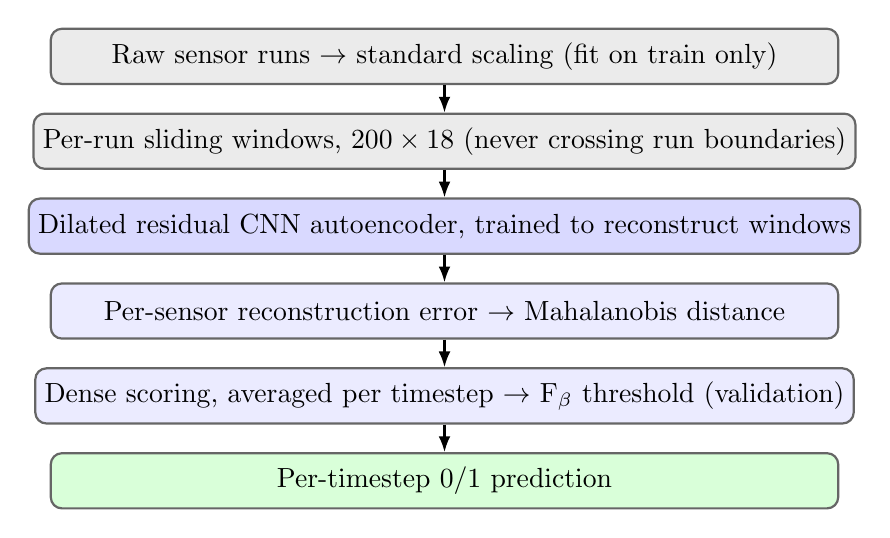
\begin{tikzpicture}[
  node distance=0.35cm,
  box/.style={rectangle, rounded corners, draw=black!60, thick, minimum width=10cm, minimum height=0.7cm, align=center},
  arr/.style={-{Latex[length=2mm]}, thick}]
\node[box, fill=black!8] (n1) {Raw sensor runs $\rightarrow$ standard scaling (fit on train only)};
\node[box, fill=black!8, below=of n1] (n2) {Per-run sliding windows, $200 \times 18$ (never crossing run boundaries)};
\node[box, fill=blue!15, below=of n2] (n3) {Dilated residual CNN autoencoder, trained to reconstruct windows};
\node[box, fill=blue!8, below=of n3] (n4) {Per-sensor reconstruction error $\rightarrow$ Mahalanobis distance};
\node[box, fill=blue!8, below=of n4] (n5) {Dense scoring, averaged per timestep $\rightarrow$ F$_\beta$ threshold (validation)};
\node[box, fill=green!15, below=of n5] (n6) {Per-timestep 0/1 prediction};
\foreach \i/\j in {1/2,2/3,3/4,4/5,5/6} \draw[arr] (n\i) -- (n\j);
\end{tikzpicture}}
\caption{Detection pipeline.}\label{fig:pipeline}
\end{figure}

\subsection{Preprocessing and Windowing}

A standard scaler is fitted on the training runs only and applied to all splits. Each run is cut into windows of $T = 200$ timesteps across all $D = 18$ sensors. Windows are built per run and never span two runs. Training windows use stride 10. Validation and test windows use stride 1, and the score of a timestep is the mean score of all windows containing it, which yields exactly one score per timestep.

\subsection{Dilated Convolutional Autoencoder}

The encoder stacks four residual blocks with dilations 1, 2, 4 and 8. Each block has two 1D convolutions (kernel size 3) with batch normalisation and ReLU, and a residual connection (a $1\times1$ convolution when channel counts differ). Channel widths are 32, 32, 32 and 64. Max-pooling by a factor of 2 forms the bottleneck ($64 \times 100$). The decoder upsamples with a transposed convolution to $32 \times 200$, applies two residual blocks with dilations 4 and 2, and projects back to 18 channels with a final convolution.

The encoder's receptive field is 61 timesteps. This wide context matters because the anomalies in this process are mostly slow drifts rather than one-step spikes. The bottleneck prevents the network from learning the identity map, which would also reconstruct anomalies well.

Training uses mean-squared reconstruction loss, Adam (learning rate $10^{-3}$), batch size 64 and up to 50 epochs. Training loss falls steadily without a plateau, while validation quality is not monotonic in the epoch count, so we evaluate every 5 epochs and keep the checkpoint with the best validation F$_\beta$.

\subsection{Per-Sensor Mahalanobis Scoring}

A flat mean-squared error averages all sensors, so a large error on one precise sensor is diluted by ordinary noise on the other 17. We instead keep one error value per sensor. For window $w$, let $e_w \in \mathbb{R}^{18}$ hold the mean squared reconstruction error of each sensor over the window. We fit a Gaussian model of normal error with mean $\mu$ and covariance $\Sigma$, where $\Sigma$ is estimated with Ledoit--Wolf shrinkage~\cite{ledoit2004well}, and score each window by
\begin{equation}
  s(w) = (e_w - \mu)^\top \Sigma^{-1} (e_w - \mu).
\end{equation}
$\mu$ and $\Sigma$ are fitted on validation windows whose labels are all normal. Section~\ref{sec:reliability} examines the effect of this choice.

\subsection{Threshold Selection}

Normal and anomalous scores overlap, and thresholds that maximise F1 on validation flagged a large share of timesteps. We therefore sweep the precision--recall curve on validation and select the threshold that maximises F$_\beta$ with $\beta = 0.5$, which weights precision more heavily than recall. We also report ROC-AUC, which measures ranking quality independently of the threshold.

%======================================================================
\section{Results}
%======================================================================

Unless stated otherwise, numbers are validation metrics. Seeds are fixed at 42, yet repeated runs of an identical configuration vary by about $\pm 0.02$ F1 (observed range 0.568--0.611), so smaller differences are not evidence of improvement.

\subsection{Current Best Result}

% TODO: UPDATE AFTER FINAL F1 OPTIMIZATION (fill the last row, or replace the
% "Current best" row once a better portal submission exists)
Table~\ref{tab:main} reports our current best submission. It scores F1 = \portalFone{} on the competition portal, slightly above its validation F1 of \valFone. Because the portal metric is not documented (Section~\ref{sec:portal}), the two numbers should not be compared directly. Work on improving the model continues; the last row of the table is reserved for the final result.

\begin{table}[ht]
\centering
\caption{Current best result. Validation metrics use the pipeline's default calibration (Section~\ref{sec:reliability}).}\label{tab:main}
\begin{tabular}{lccccc}
\toprule
Model & \multicolumn{4}{c}{Validation} & Portal \\
\cmidrule(lr){2-5}
 & F1 & Precision & Recall & ROC-AUC & F1 \\
\midrule
Current best (this paper) & \valFone & \valPrec & \valRec & \valAUC & \textbf{\portalFone} \\
Final model & \multicolumn{5}{c}{\finalFone} \\
\bottomrule
\end{tabular}
\end{table}

\subsection{Why This Design}

\paragraph{Scoring.} With the same dilated autoencoder, replacing flat mean-squared error by per-sensor Mahalanobis scoring raised validation ROC-AUC from 0.65 to 0.76 and F1 from 0.48 to the 0.58--0.61 range. Because ROC-AUC does not depend on the threshold, this reflects better separation of anomalies from normal data rather than a better cut-off.

\paragraph{Fusion.} We tested whether a detector built on different features could cover the autoencoder's blind spots, fusing it with an Isolation Forest~\cite{liu2008isolation} on per-window statistics and with a Local Outlier Factor detector~\cite{breunig2000lof} on cross-sensor features. The LOF fusion weight was chosen by 5-fold cross-validation grouped by run. In most folds the weight search selected the autoencoder alone, and the out-of-fold hybrid did not exceed the autoencoder alone. We therefore use the autoencoder without fusion.

\paragraph{Alternatives that did not help.} Table~\ref{tab:alt} lists three later changes, each evaluated on one shared trained network so that differences reflect the change rather than training noise. Choosing the threshold for F1 instead of F$_{0.5}$ raised validation F1 by 0.024, which is within run-to-run variation, and flagged 84\% of test timesteps, so we did not adopt it. Normalising each run's scores by its median and MAD lowered ROC-AUC, meaning it damaged the ranking itself. Fitting $\mu$ and $\Sigma$ on training windows lowered ROC-AUC further; training-window errors are much tighter than errors on held-out normal windows (per-sensor variance 0.000144 vs.\ 0.001727), since the network was trained on them.

\begin{table}[ht]
\centering
\caption{Alternatives evaluated on one shared network (validation). This network is a re-run of the same pipeline; its reference row differs from Table~\ref{tab:main} by run-to-run variation.}\label{tab:alt}
\begin{tabular}{lccc}
\toprule
Variant & F1 & ROC-AUC & Test flagged \\
\midrule
Reference (F$_{0.5}$ threshold) & 0.583 & 0.769 & 0.617 \\
F1-optimal threshold & 0.607 & 0.769 & 0.842 \\
Per-run median/MAD normalisation & 0.405 & 0.677 & 0.102 \\
Normal model fitted on train windows & 0.483 & 0.611 & 0.833 \\
\bottomrule
\end{tabular}
\end{table}

\subsection{Failure Analysis}

The diagnostic plots in this section come from a diagnostic re-run of the same pipeline. The scores of normal and anomalous timesteps overlap heavily at low values; this overlap is what limits ROC-AUC to about 0.76, and no choice of threshold removes it. Figure~\ref{fig:sensors} shows that the error signal comes mainly from flow and pressure sensors (FT703, T703, FT704, PDI702, FYI702), while some sensors show almost no difference between normal and anomalous windows. Figure~\ref{fig:timelines} shows the per-run behaviour: in two validation runs the score peaks coincide with the labelled anomalies but stay below the global threshold, because score magnitudes differ by about two orders of magnitude between runs, and both runs score F1 = 0.

\begin{figure}[t]
\centering
\plot{figures/per_sensor_error.png}{width=\linewidth}
\caption{Mean per-sensor reconstruction error on normal and anomalous validation windows (diagnostic re-run).}\label{fig:sensors}
\end{figure}

\begin{figure}[t]
\centering
\plot{figures/val_score_timelines.png}{width=\linewidth}
\caption{Anomaly score over time for each validation run, with labelled anomalies shaded and the global threshold shown (diagnostic re-run).}\label{fig:timelines}
\end{figure}

\subsection{Ongoing Optimisation}

% TODO: UPDATE AFTER FINAL F1 OPTIMIZATION (describe final experiments here)
\finalResults

%======================================================================
\section{How Reliable Are the Numbers?}\label{sec:reliability}
%======================================================================

\subsection{Same-Run Calibration Is Optimistic}

The Mahalanobis model is fitted on normal windows from the same validation runs it then scores, which test runs can never provide. To measure the effect, we re-scored each validation run with a model fitted only on the other nine runs (leave-one-run-out, Table~\ref{tab:loro}), using the same network as Table~\ref{tab:alt}.

\begin{table}[ht]
\centering
\caption{Effect of leave-one-run-out (LORO) calibration of the Mahalanobis model (validation).}\label{tab:loro}
\begin{tabular}{lcccc}
\toprule
Calibration & ROC-AUC & F1 & Precision & Recall \\
\midrule
Same runs (pipeline default) & 0.769 & 0.583 & 0.577 & 0.589 \\
Leave-one-run-out & 0.699 & 0.525 & 0.462 & 0.609 \\
\bottomrule
\end{tabular}
\end{table}

ROC-AUC falls by 0.070 and F1 by 0.058, and ROC-AUC decreases in all ten runs. The validation figures in Table~\ref{tab:main} are therefore optimistic, and future comparisons should use run-grouped validation.

\subsection{What Does the Portal Measure?}\label{sec:portal}

The current best submission flags 62.2\% of test timesteps. If the portal computed point-wise F1, a submission that flags a fraction $q$ of timesteps, on a test set with prevalence $p$, at recall $r$, would score
\begin{equation}
  F_1 = \frac{2\,r\,p}{q + p}.
\end{equation}
With $q = 0.622$ and the validation prevalence $p = 0.2395$, even perfect recall gives at most 0.556. Reaching \portalFone{} requires $p \geq 0.286$ at perfect recall, or $p \geq 0.44$ at the validation recall of 0.76. Either the test set contains far more anomalies than the validation set, or the portal uses a different metric, such as point-adjusted or event-wise F1, which are known to reward generous flagging~\cite{kim2022towards}. Until this is known, portal scores cannot be read as point-wise F1, and threshold choices for the portal remain uncertain.

%======================================================================
\section{Conclusion}
%======================================================================

% TODO: UPDATE AFTER FINAL F1 OPTIMIZATION
A dilated residual autoencoder with per-sensor Mahalanobis scoring detects anomalies in unlabelled 18-sensor process data, reaching F1 = \portalFone{} on the competition portal (validation F1 = \valFone). Final result: \finalFone. The scoring method contributed more than any change to the network, and fusion with tabular detectors did not help. Leave-one-run-out calibration shows that the standard validation estimate is optimistic. Ongoing work targets the overlap between normal and anomalous scores, for example by down-weighting likely anomalies in the unlabelled training data and averaging over training seeds, and aims to establish which metric the portal computes before tuning thresholds further.

\begin{credits}
\subsubsection{\ackname}
Experiments were run on the RPTU Elwetritsch cluster.

\subsubsection{\discintname}
The authors have no competing interests to declare that are relevant to the content of this article.
\end{credits}

\bibliographystyle{splncs04}
\bibliography{references}

\end{document}
